% DP-ProtOn: Dirichlet-Process-Guided Online Prototype Learning for Continual Classification
% TMLR submission draft — compile with xelatex
\documentclass[11pt,a4paper]{article}

% ── Packages ──
\usepackage{fontspec}
\usepackage[hmargin=2.5cm,vmargin=2.5cm]{geometry}
\usepackage{amsmath,amssymb}
\usepackage{graphicx}
\usepackage{booktabs}
\usepackage{caption}
\usepackage{hyperref}
\usepackage{xcolor}
\usepackage{enumitem}
\usepackage{float}

\hypersetup{colorlinks=true,linkcolor=blue,citecolor=blue,urlcolor=blue}
\captionsetup{font=small,labelfont=bf}

% ── Math operators ──
\DeclareMathOperator*{\logsumexp}{logsumexp}
\DeclareMathOperator*{\argmax}{arg\,max}

% ── Title ──
\title{\textbf{DP-ProtOn: Dirichlet-Process-Guided Online Prototype Learning for Continual Classification}}
\author{Feng Yuhan}
\date{}

\begin{document}
\maketitle

% ======================================================================
% Correction notice — added 2026-10-11
% ======================================================================
\begin{center}
\fbox{\parbox{0.94\textwidth}{%
\textbf{\color{red!70!black}Correction (2026-10-11): the \S5.2 creation-rule comparison does not hold.}
The headline ablation of this paper --- that the CRP criterion beats a distance-threshold online
$k$-means by $\Delta$ACC${}=0.6960\pm0.0528$ at matched prototype budget, and that therefore
``the DP criterion is necessary, not excess complexity'' --- is an artifact of a confounded
comparison. The two models did not differ only in their creation rule: the threshold $k$-means
baseline allocated basins \textbf{label-blind} (searching all centres regardless of class) while
DP/CRP's rejection baseline carried a \textbf{per-class} base measure, and the baseline's
threshold was not calibrated to a structural target. Re-measured on the same dataset (sklearn
\textit{digits}, 20 basins, matched budget), with each criterion's single scalar hyperparameter
fixed by a structural target and one no-knob readout for all four:
\begin{center}
\begin{tabular}{lc}
\toprule
Criterion & ACC @ 20 basins \\
\midrule
hard threshold & 0.916 \\
threshold online $k$-means & \textbf{0.935} \\
DP / CRP (estimated base) & 0.917 \\
DP / CRP (fixed prior base) & 0.916 \\
\bottomrule
\end{tabular}
\end{center}
The DP figure reproduces ($0.9303 \rightarrow 0.917$); the \textbf{baseline} moved from $0.2342$
to $0.935$. Across every real dataset tested the spread between all four criteria is $\le 1.9$
accuracy points, with no consistent winner. Treat \S5.2 and the abstract's $\Delta$ACC figure as
superseded. What still stands: the per-class architecture, the denoised in-basin centroid, the
rank/density readout, and exact local deletion. What does not: the necessity claim for DP/CRP
basin creation. The re-measurement is in the companion repository \texttt{Fengrru/energy-basin-cl}.
}}
\end{center}

% ======================================================================
\section{Abstract}
% ======================================================================

We study rehearsal-free, single-pass continual classification on top of frozen features, and ask a deliberately narrow question: \textit{given a good creation criterion and a good readout, how far can a purely online prototype learner go, and which of its components actually matter?} We introduce \textbf{DP-ProtOn} (Dirichlet-Process-guided Prototype Online learner), a lightweight model with three components: (i)~class-conditional Gaussian ``basins'' allocated on the fly using a Chinese-Restaurant-Process (CRP) creation criterion with diagonal covariance, (ii)~one online denoised centroid per basin maintained via competitive-learning mean updates, and (iii)~a Parzen / soft-$k$NN density readout over those centroids. DP-ProtOn emerged from the systematic falsification of a more elaborate energy-attractor design whose energy-softmin routing proved \textit{net-negative} in high dimensions — a same-model readout ablation pins this failure precisely. All headline claims carry multi-seed variance: across 5 seeds on sklearn \textit{digits} and 3 seeds on \textit{Split-MNIST}, the CRP criterion beats a distance-threshold online $k$-means by $\Delta\text{ACC}=0.6960\pm0.0528$ at matched prototype budget (Figure~1a), online denoised centroids beat offline $k$-means at equal budget by $0.0340\pm0.0053$ (Figure~1b), and on Split-MNIST DP-ProtOn reaches $0.8747\pm0.0019$ ACC with near-zero forgetting ($\text{BWT}=-0.0471\pm0.0049$), a $+0.20$ ACC advantage with $8\times$ better backward transfer over Experience Replay at equal memory (Figure~1c), while EWC and fine-tuning collapse ($\text{BWT}\approx-0.99$). Critically, because each class is a spatially localized, label-tagged attractor, DP-ProtOn supports \textbf{training-free knowledge editing}: deleting, relabeling, and injecting classes are $O(1)$ set operations on the basin list. We verify all three surgeries across 5 seeds (Figure~2): deletion drops the target class to 0.0000 ACC while perturbing others by $\le 0.0467$; relabeling is byte-identical in decision geometry ($1.0000\pm0.0000$); and injecting a held-out class from merely 20 samples recovers $0.8564\pm0.0603$ ACC with no measurable forgetting of old classes. We position DP-ProtOn as an honest, fully-ablated baseline and as evidence that prototype attractors are directly editable knowledge units — a property softmax classifiers categorically lack.

% ======================================================================
\section{Introduction}
% ======================================================================

Continual learning (CL) asks a model to absorb a non-stationary stream of tasks without \textit{catastrophic forgetting} of what it learned before. The dominant strategies are: \textbf{regularization} that penalizes weight drift via a surrogate importance measure (EWC; Kirkpatrick et al., 2017), \textbf{rehearsal} that interleaves stored exemplars with new data (Chaudhry et al., 2019), and \textbf{architectural growth} that freezes old parameters and appends new capacity. A separate, older line of work — prototype and nearest-class-mean (NCM) classifiers — sidesteps gradient interference entirely by \textit{storing} class-condensed summaries and classifying by similarity. These methods are attractive for CL precisely because adding a class does not overwrite the parameters that encode existing classes: there are no parameters to overwrite.

This paper is a careful, negative-result-inclusive study of one such prototype learner. Our starting point was an ambitious energy-based design — a ``Precision-Weighted Attractor Field Machine'' (PW-AFM) with radial potential wells, softmin energy routing across basins, precision gating, inter-basin barrier terms, and reversible decay. The hypothesis was that an energy landscape over basins would deliver principled continual learning. \textbf{That hypothesis did not survive contact with high-dimensional data.} Rather than discard the project, we treated the failed design as an ablation target and asked: \textit{which components actually carry the performance, and which are dead weight?}

The answer is surprisingly compact. Only three ingredients survive systematic ablation:

\begin{enumerate}[label=(\arabic*),leftmargin=*]
\item \textbf{A Dirichlet-Process / CRP creation criterion} with \textit{diagonal} covariance that compares a rich-get-richer class-conditional likelihood $\log n_i + \log\mathcal{N}(x \mid c_i,\Sigma_i)$ against a universal rejection baseline $\log\alpha + \log p_0(x)$.
\item \textbf{One online denoised centroid per basin}, updated by a running competitive mean, replacing noisy raw memory samples.
\item \textbf{A Parzen / soft-$k$NN density readout} that classifies via log-sum-exp over centroids, replacing the failed energy-softmin.
\end{enumerate}

Everything else — energy routing, full covariance, per-basin mini-GMMs, barrier terms, the precision gate — is either net-negative or negligible for classification and is removed. We call the resulting compact model \textbf{DP-ProtOn}.

Our contributions are concrete and diagnostic:

\begin{itemize}[leftmargin=*]
\item \textbf{A same-model readout ablation} (Section~5.1) that pins the energy-routing failure precisely: on \textit{identical} trained basins, switching from energy-softmin (0.751) to a local density readout (0.887) yields a large jump, proving the basins store useful structure that the energy mechanism fails to exploit. The culprit is distance concentration in 30–64~D (Beyer et al., 1999).
\item \textbf{A controlled necessity test for the DP criterion} (Section~5.2; Figure~1a). Holding the readout and centroid machinery fixed and varying \textit{only} the creation rule, DP beats distance-threshold online $k$-means by $\Delta=0.696\pm0.053$ (5 seeds) at matched prototype budget, and even beats it at $8\times$ the threshold budget in single-seed sweeps.
\item \textbf{Multi-seed continual-learning results} (Section~5.4; Figure~1c). On Split-MNIST (3 seeds, frozen 50-D features), DP-ProtOn reaches $0.8747\pm0.0019$ ACC with $\text{BWT}=-0.047\pm0.005$, beating Experience Replay at equal memory by $+0.20$ ACC and $8\times$ better backward transfer. EWC and fine-tuning collapse ($\text{BWT}\approx-0.99$).
\item \textbf{Training-free knowledge editing} (Section~5.5; Figure~2). Because basins are discrete, label-tagged attractors, deleting, relabeling, and injecting classes are $O(1)$ set operations — a capability that softmax classifiers categorically lack.
\end{itemize}

We deliberately scope out feature learning and rehearsal: DP-ProtOn operates on frozen features and stores no replay buffer. This makes it a clean, reproducible baseline rather than a state-of-the-art claim.

% ======================================================================
\section{Related Work}
% ======================================================================

\textbf{Prototype and nearest-class-mean continual learning.} iCaRL (Rebuffi et al., 2017) stores exemplars selected via herding and classifies by nearest-mean, combined with knowledge distillation. End-to-End Incremental Learning (Castro et al., 2018) and BiC (Wu et al., 2019) add learned bias-correction layers on top of exemplar-based nearest-mean. All three require gradient updates and tuned distillation hyperparameters. The closest ancestor to our readout is pure nearest-class-mean classification (Mensink et al., 2013). DP-ProtOn is simpler: no distillation, no gradient-based class learning, and centroids are produced by a purely online competitive mean rather than by selecting exemplars.

\textbf{Online and streaming clustering.} Streaming $k$-means (Sculley, 2010), BIRCH (Zhang et al., 1996), and DenStream (Cao et al., 2006) grow cluster structure online. The critical distinguishing element of DP-ProtOn is the \textit{creation criterion}: instead of a fixed distance threshold, it employs a Bayesian-nonparametric CRP rule with per-basin covariance. Our control experiment (Section~5.2) shows this difference is decisive.

\textbf{Bayesian nonparametrics.} The Dirichlet Process (Ferguson, 1973; Teh, 2010) and its CRP representation (Blackwell \& MacQueen, 1973) provide a principled rich-get-richer prior over an unbounded number of components. We use the CRP not for full posterior inference but as a lightweight, adaptive, covariance-aware \textit{allocation} rule at streaming time.

\textbf{Regularization- and rehearsal-based methods.} EWC (Kirkpatrick et al., 2017) anchors weights via a Fisher-information penalty; Experience Replay (Chaudhry et al., 2019; Aljundi et al., 2019) interleaves stored exemplars. On frozen features these gradient-based methods are brittle, and our results (Section~5.4) reproduce that fragility.

\textbf{Energy-based models.} Our design originated in the EBM tradition (LeCun et al., 2006). Our core negative finding — that energy-softmin degrades in high dimensions due to distance concentration (Beyer et al., 1999) and is dominated by a local density readout — is a concrete, empirically grounded contribution.

% ======================================================================
\section{Method}
% ======================================================================

\subsection{Overview and pipeline}

DP-ProtOn maintains a set of \textbf{basins} $\{B_i\}_{i=1}^{K}$. Each basin $B_i$ consists of: a class label $\ell_i$, a running sample count $n_i$, a running Gaussian summary $(c_i,\Sigma_i)$ with diagonal $\Sigma_i$ used \textit{exclusively} for the CRP creation decision, and a small set of \textbf{online denoised centroids} $\{m_{ik}\}_{k=1}^{K_i}$ used \textit{exclusively} for classification. Features are frozen: we fit PCA-whitening once on a pretraining pool (30\% of training data) and never update it. The BWT metric follows Lopez-Paz \& Ranzato (2017). Table~\ref{tab:notation} summarizes key notation.

\medskip\noindent
{\small
\begin{tabular}{@{}ll@{}}
\toprule
Symbol & Meaning \\
\midrule
$\mathcal{B}=\{B_i\}_{i=1}^K$ & Set of all basins \\
$\ell_i\in\mathcal{Y}$ & Class label of basin $i$ \\
$n_i\in\mathbb{N}$ & Number of points assigned to basin $i$ \\
$c_i\in\mathbb{R}^d$ & Online mean (centroid) of basin $i$ \\
$\Sigma_i=\operatorname{diag}(\sigma_{i1}^2,\ldots,\sigma_{id}^2)$ & Diagonal covariance of basin $i$ \\
$m_{ik}\in\mathbb{R}^d$ & $k$-th online denoised sub-centroid of basin $i$ \\
$\alpha>0$ & CRP concentration parameter \\
$p_0(x)=\mathcal{N}(x\mid 0,\sigma_0^2\cdot\text{base\_scale}^2)$ & Universal reference (base measure proxy) \\
$h>0$ & Parzen kernel bandwidth \\
\bottomrule
\end{tabular}
\captionof{table}{Key notation.}\label{tab:notation}}

\medskip\noindent
\fbox{\begin{minipage}{0.95\textwidth}
\textbf{Algorithm 1:} DP-ProtOn stream step (single point $(x,y)$).\\[2pt]
\textbf{1. Candidate selection.} Let $\mathcal{B}_y = \{B \in \mathcal{B} : \ell_B = y\}$. If $\mathcal{B}_y = \emptyset$, go to step~3.\\
\textbf{2. CRP scoring.} For each $B \in \mathcal{B}_y$: $s_B = \log n_B + \log\mathcal{N}(x \mid c_B, \Sigma_B)$.\\
Let $B^* = \argmax_{B \in \mathcal{B}_y} s_B$. Compute rejection baseline: $s_0 = \log\alpha + \log p_0(x)$.\\
If $s_{B^*} > s_0$, assign $x$ to $B^*$ (step~4); else create new basin (step~3).\\
\textbf{3. Create basin.} New basin with label $y$, $n=1$, $c=x$, $\Sigma=\sigma_0^2 I$, centroid $m=x$.\\
\textbf{4. Update.} $n_B \mathrel{+}= 1$, $c_B \leftarrow c_B + (x-c_B)/n_B$, update $\Sigma_B$, update nearest centroid: $n_{Bk} \mathrel{+}= 1$, $m_{Bk} \mathrel{+}= (x-m_{Bk})/n_{Bk}$.
\end{minipage}}

\subsection{CRP basin creation: design rationale}

The CRP score follows from the Dirichlet Process mixture model posterior predictive distribution. Under a DP prior with concentration parameter $\alpha$ and base measure $G_0$, the conditional probability of assigning a new point to an existing component $i$ (given all previous assignments) is proportional to $n_i$ --- the \textbf{rich-get-richer} property --- while the probability of instantiating a new component is proportional to $\alpha$. Equipping each component with a Gaussian likelihood $\mathcal{N}(\cdot\mid c_i,\Sigma_i)$ yields the log-posterior predictive score:

\[
\log p(\text{assign to } B_i \mid x, \text{history})
\propto \log n_i + \log\mathcal{N}(x \mid c_i, \Sigma_i) = s_i.
\]

The rejection baseline $s_0 = \log\alpha + \log p_0(x)$ is the log-probability of creating a new basin, where $p_0(x)=\mathcal{N}(x\mid 0,\sigma_0^2\cdot\text{base\_scale}^2)$ approximates the DP base measure $G_0$. The decision rule $s_{B^*} > s_0$ thus implements Bayesian model selection between two hypotheses: ``assign to the best-matching existing same-class basin'' versus ``instantiate a new basin from the prior.''

Three properties distinguish this from a fixed distance threshold:
\begin{enumerate}[label=(\arabic*),leftmargin=*]
\item \textbf{Covariance-adaptive acceptance.} The per-dimension variance $\Sigma_i$ makes the acceptance region ellipsoidal and data-adaptive, rather than a fixed-radius hypersphere. A basin covering a tightly clustered mode has small variance and accepts points only in its immediate neighborhood; a basin over a diffuse region automatically widens.
\item \textbf{Universal contamination guard.} The candidate set is restricted to $\mathcal{B}_y = \{B\in\mathcal{B}:\ell_B=y\}$, so a point from class~A is never silently absorbed into a basin for class~B. The rejection baseline $s_0$ provides a data-independent threshold for genuinely novel classes.
\item \textbf{Automatic budget control.} The $\log n_i$ term penalizes singleton basins and encourages merging, while $\alpha$ directly controls the expected basin count: $\mathbb{E}[K] \approx \alpha\log(1 + N/\alpha)$ (Antoniak, 1974). In practice, $\alpha{=}1.0$ yields $\approx$10 basins for digits; $\alpha{=}10^4$ yields $\approx$30 for the synthetic 30-mode dataset.
\end{enumerate}

We use \textbf{diagonal} $\Sigma_i$ throughout. In the small-data, high-dimensional regime typical of online learning, full covariance estimates are ill-conditioned: the $\mathcal{O}(d^2)$ parameters per basin require sample sizes that streaming never provides. The diagonal parameterization needs only $d$ variance parameters and stabilizes quickly from few observations. Single-seed ablation confirms this is not merely conservative but essential: diagonal~0.746 vs full~0.680 at $d{=}30$, and full covariance degrades to near-random allocation at $d{=}64$.

\subsection{Online denoised centroids (sub-centroids)}

Each basin maintains $K_i=$ \texttt{n\_sub} centroids updated via competitive learning: an incoming point $x$ assigned to basin $i$ is routed to the nearest centroid by Euclidean distance, and that centroid is moved toward $x$:

\[
n_{ik} \mathrel{+}= 1, \qquad m_{ik} \mathrel{+}= \frac{x - m_{ik}}{n_{ik}}.
\]

This is a Robbins-Monro stochastic approximation (Robbins \& Monro, 1951) with step size $\eta_t = 1/t$ at the $t$-th update to centroid $k$. The sequence $\{\eta_t\}$ satisfies the standard convergence conditions $\sum_t \eta_t = \infty$, $\sum_t \eta_t^2 < \infty$, guaranteeing almost-sure convergence to $\mathbb{E}[x \mid \text{basin } i]$ under mild regularity (bounded variance, i.i.d.~stream). Crucially, this requires \textit{no learning-rate tuning} --- the step size is fully determined by the assignment count.

With \texttt{n\_sub=1} (the practical default), each basin is represented by a single running mean. Why does this beat offline $k$-means at equal prototype budget ($\Delta=0.0340\pm0.0053$, Section~5.3)? Two reasons: (i)~the online mean converges \textit{toward} the data-generating distribution continuously, while Lloyd clustering on a finite static sample is biased by class imbalance and random initialization; (ii)~each $O(1/n_i)$ update contributes diminishing noise, providing implicit regularization that prevents overfitting to early observations --- a property that offline batch clustering lacks. With \texttt{n\_sub}$>$1, multiple centroids per basin capture multi-modal within-class structure, closing the gap to the 1-NN upper bound at the cost of additional prototypes.

\subsection{Density readout (Parzen / soft-$k$NN)}

Classification scores a query $x$ against all basin centroids via log-sum-exp with bandwidth $h$:

\[
s_i(x) = \logsumexp_{k=1}^{K_i} \left(-\frac{1}{2} \frac{\lVert x - m_{ik}\rVert^2}{h^2}\right), \qquad
\hat{y}(x) = \ell_{\argmax_i \; s_i(x)}.
\]

This local, prototype-anchored readout avoids the distance concentration that cripples global energy-softmin. The bandwidth $h$ is robust: ACC varies only within $\approx$0.013 over $h\in[0.3,2.0]$.

\subsection{Knowledge editing interface}

Because knowledge in DP-ProtOn lives in discrete, label-tagged, spatially localized attractors:

\begin{itemize}[leftmargin=*]
\item \textbf{Delete} class $\ell$: remove every basin with $\ell_i=\ell$. $O(|\mathcal{B}|)$.
\item \textbf{Relabel} $\ell\to\ell'$: reassign $\ell_i \leftarrow \ell'$. Geometry untouched — decision surface is byte-identical up to the label map.
\item \textbf{Inject} new class: stream $N$ labeled examples through Algorithm~1. CRP allocates fresh basins without disturbing existing ones.
\end{itemize}

A softmax MLP cannot perform any of these without retraining the entire network, because every class is entangled in $W\in\mathbb{R}^{C\times d}$.

\subsection{Computational properties}

All operations are lightweight and streaming-compatible. For a stream of $N$ points in $\mathbb{R}^d$ with $K$ active basins:

\begin{itemize}[leftmargin=*]
\item \textbf{CRP scoring:} $O(K_y d)$ per point, where $K_y = |\mathcal{B}_y|$ is the number of same-class basins (typically $K_y \ll K$). The Gaussian log-likelihood requires only $d$ operations due to diagonal $\Sigma_i$, avoiding the $O(d^3)$ determinant and inverse of a full covariance.
\item \textbf{Centroid update:} $O(d)$ per assigned point --- a single vector difference and scalar division.
\item \textbf{Readout (classification):} $O(K d)$ per query via log-sum-exp over all centroids. With \texttt{n\_sub=1}, $K$ equals the number of basins, typically 10--50, making each classification sub-microsecond for $d \le 64$.
\item \textbf{Memory:} $O(K d)$ floats for centroids and diagonal variances. At $K \approx 30$, $d = 50$, this is $\approx$3,000 floats ($<$12 KB) --- orders of magnitude below any gradient-based method.
\item \textbf{Knowledge editing:} $O(|\mathcal{B}|)$ for delete/relabel (single list scan); $O(N K_y d)$ for inject (stream $N$ new examples through CRP).
\end{itemize}

The full system is implemented in $\approx$340 lines of pure Python + NumPy with no GPU dependency, no automatic differentiation framework, and no batch processing. Inference throughput exceeds $10^5$ points/second on a single CPU core for $d \le 64$, and the streaming training cost per point is $<$$1\mu$s.

\subsection{Hyperparameters and default configuration}

\begin{table}[H]
\centering
\caption{DP-ProtOn hyperparameters, defaults, and sensitivity.}
\begin{tabular}{@{}llll@{}}
\toprule
Parameter & Default & Role & Sensitivity \\
\midrule
\texttt{create\_rule} & \texttt{'dp'} & Basin creation mechanism & Must-use: threshold is far worse \\
\texttt{dp\_alpha} & 1.0 / $10^4$ & CRP concentration & Monotonic basin count control \\
\texttt{dp\_diag\_cov} & \texttt{True} & Diagonal covariance in CRP & Essential: full cov fails in high-D \\
\texttt{base\_scale} & 3.0 & Reference-baseline width & Wider = fewer basins \\
\texttt{readout} & \texttt{'density'} & Classification mechanism & Density $\gg$ energy \\
\texttt{n\_sub} & 1 & Centroids per basin & $k{=}1$ is efficiency sweet spot \\
\texttt{density\_bw} & 1.0 & Parzen kernel bandwidth & Robust across [0.3, 2.0] \\
\texttt{T} & 0.3 & Temperature (legacy) & Unused in density readout \\
\texttt{sigma0} & 1.0 & Initial $\Sigma$ scale & Sets length scale \\
\bottomrule
\end{tabular}
\end{table}

Removed components (verified-unhelpful for classification): energy-softmin routing, full covariance, per-basin mini-GMM, barrier terms, precision gate, reversible decay.

% ======================================================================
\section{Experimental Setup}
% ======================================================================

\subsection{Datasets and preprocessing}

All datasets are projected into a frozen feature space via PCA followed by whitening (zero-mean, unit-variance per dimension). The PCA transform is fit once on a pretraining pool (30\% of training data, stratified by class) and held fixed for all subsequent experiments --- no method is permitted to update the feature representation.

\begin{itemize}[leftmargin=*]
\item \textbf{Digits} (sklearn \texttt{load\_digits}; Pedregosa et al., 2011): 1,797 $8\times8$ grayscale images across 10 classes (0--9), roughly class-balanced ($\approx$180/class). PCA-whitened from 64-D raw pixel intensities to $d{=}30$ (retaining $>$95\% of variance). Train/test split: 70/30, stratified by class. Used for creation-rule ablation (Section~5.2), prototype-source ablation (Section~5.3), knowledge editing (Section~5.5), and all single-seed supporting ablations (Section~5.6).

\item \textbf{Split-MNIST} (LeCun et al., 1998): The full MNIST training set (60,000 $28\times28$ images) is partitioned into 5 sequential tasks of 2 classes each: \{0,1\}, \{2,3\}, \{4,5\}, \{6,7\}, \{8,9\}. Each image is flattened to 784-D, then PCA-whitened to $d{=}50$ (retaining $>$90\% of variance). The standard 10,000-image MNIST test set is used for evaluation on all classes seen so far after each task. Used for continual learning benchmarks (Section~5.4).

\item \textbf{Synthetic multi-modal} (\texttt{sklearn.make\_classification}): 6,000 points in $d{=}50$ with 10 classes $\times$ 3 informative subclusters per class = 30 true modes, plus 47 noise dimensions. Designed to stress-test whether DP-ProtOn can recover the true mode structure from a single streaming pass without access to the ground-truth subcluster labels. The 10-class labels are used for training; the 30-mode structure is known only to the oracle offline $k$-means baseline. Used for multi-modal scaling analysis (Section~5.6).
\end{itemize}

\subsection{Continual learning protocol}

All experiments use a \textbf{5-task sequential protocol}: tasks arrive one at a time, each introducing 2 new classes (total 10 classes after task~5). After each task, the model is evaluated on all classes seen so far. Metrics follow Lopez-Paz \& Ranzato (2017):
\begin{itemize}[leftmargin=*]
\item \textbf{ACC} (average accuracy): mean per-class accuracy over all classes seen after the final task.
\item \textbf{BWT} (Backward Transfer): $\text{BWT} = \frac{1}{T-1}\sum_{t=1}^{T-1} (R_{T,t} - R_{t,t})$, where $R_{T,t}$ is the accuracy on task $t$ after training on all $T$ tasks, and $R_{t,t}$ is the accuracy on task $t$ immediately after learning it. Negative BWT indicates forgetting; zero BWT indicates perfect retention.
\end{itemize}

\subsection{Multi-seed methodology}

Every headline claim is reported as mean$\pm$standard deviation over multiple independent runs with different random seeds, controlling for: (i)~train/test split variation, (ii)~data ordering within each task, (iii)~task ordering (for Split-MNIST, the task sequence is fixed but within-task ordering varies). Headline results use \textbf{5 seeds} (0--4) on digits and \textbf{3 seeds} (0--2) on Split-MNIST (the PyTorch baselines --- EWC, Replay, Joint, Fine-tuning --- each train a 256-hidden-unit MLP per task per seed, making 3 seeds the practical limit on CPU).

For the creation-rule control (Section~5.2), the threshold $k$-means budget is re-matched per seed: the threshold $\tau$ is tuned so that the average prototype count across seeds matches DP-ProtOn's to within $\pm$1 prototype --- comparison is always at equal budget. Features are re-fit per seed. Single-seed results in Sections~5.1 and~5.6 are explicitly labeled as such.

\subsection{Baselines}

All baselines share identical frozen PCA-whitened features with DP-ProtOn. Gradient-based baselines use a 2-layer MLP (256 hidden units, ReLU activation, cross-entropy loss, SGD with lr=0.01, momentum=0.9, batch size=32). EWC uses $\lambda{=}1000$, selected from $\{10^2,10^3,10^4\}$ as best on a held-out validation split. Experience Replay stores 240 exemplars (24/class after task~5), matching DP-ProtOn's $\approx$240-float memory budget. Non-gradient baselines operate directly on the frozen features with no learnable parameters.

\begin{table}[H]
\centering
\caption{Baselines at matched frozen features.}
\begin{tabular}{@{}lll@{}}
\toprule
Baseline & Description & Gradient? \\
\midrule
Joint & Train MLP on all tasks jointly & Yes --- oracle \\
Experience Replay & 240 exemplars, replay with new data & Yes \\
EWC ($\lambda{=}1000$) & Fisher penalty on weights & Yes \\
Fine-tuning & Sequential MLP, no mitigation & Yes --- lower bound \\
Offline $k$-means-30 & Lloyd clustering, 3 centroids/class & No \\
1-NN & Store all points, nearest neighbor & No --- upper bound \\
Threshold $k$-means & Online $k$-means, distance-threshold creation & No --- DP twin \\
\bottomrule
\end{tabular}
\end{table}

% ======================================================================
\section{Results}
% ======================================================================

\begin{figure}[H]
\centering
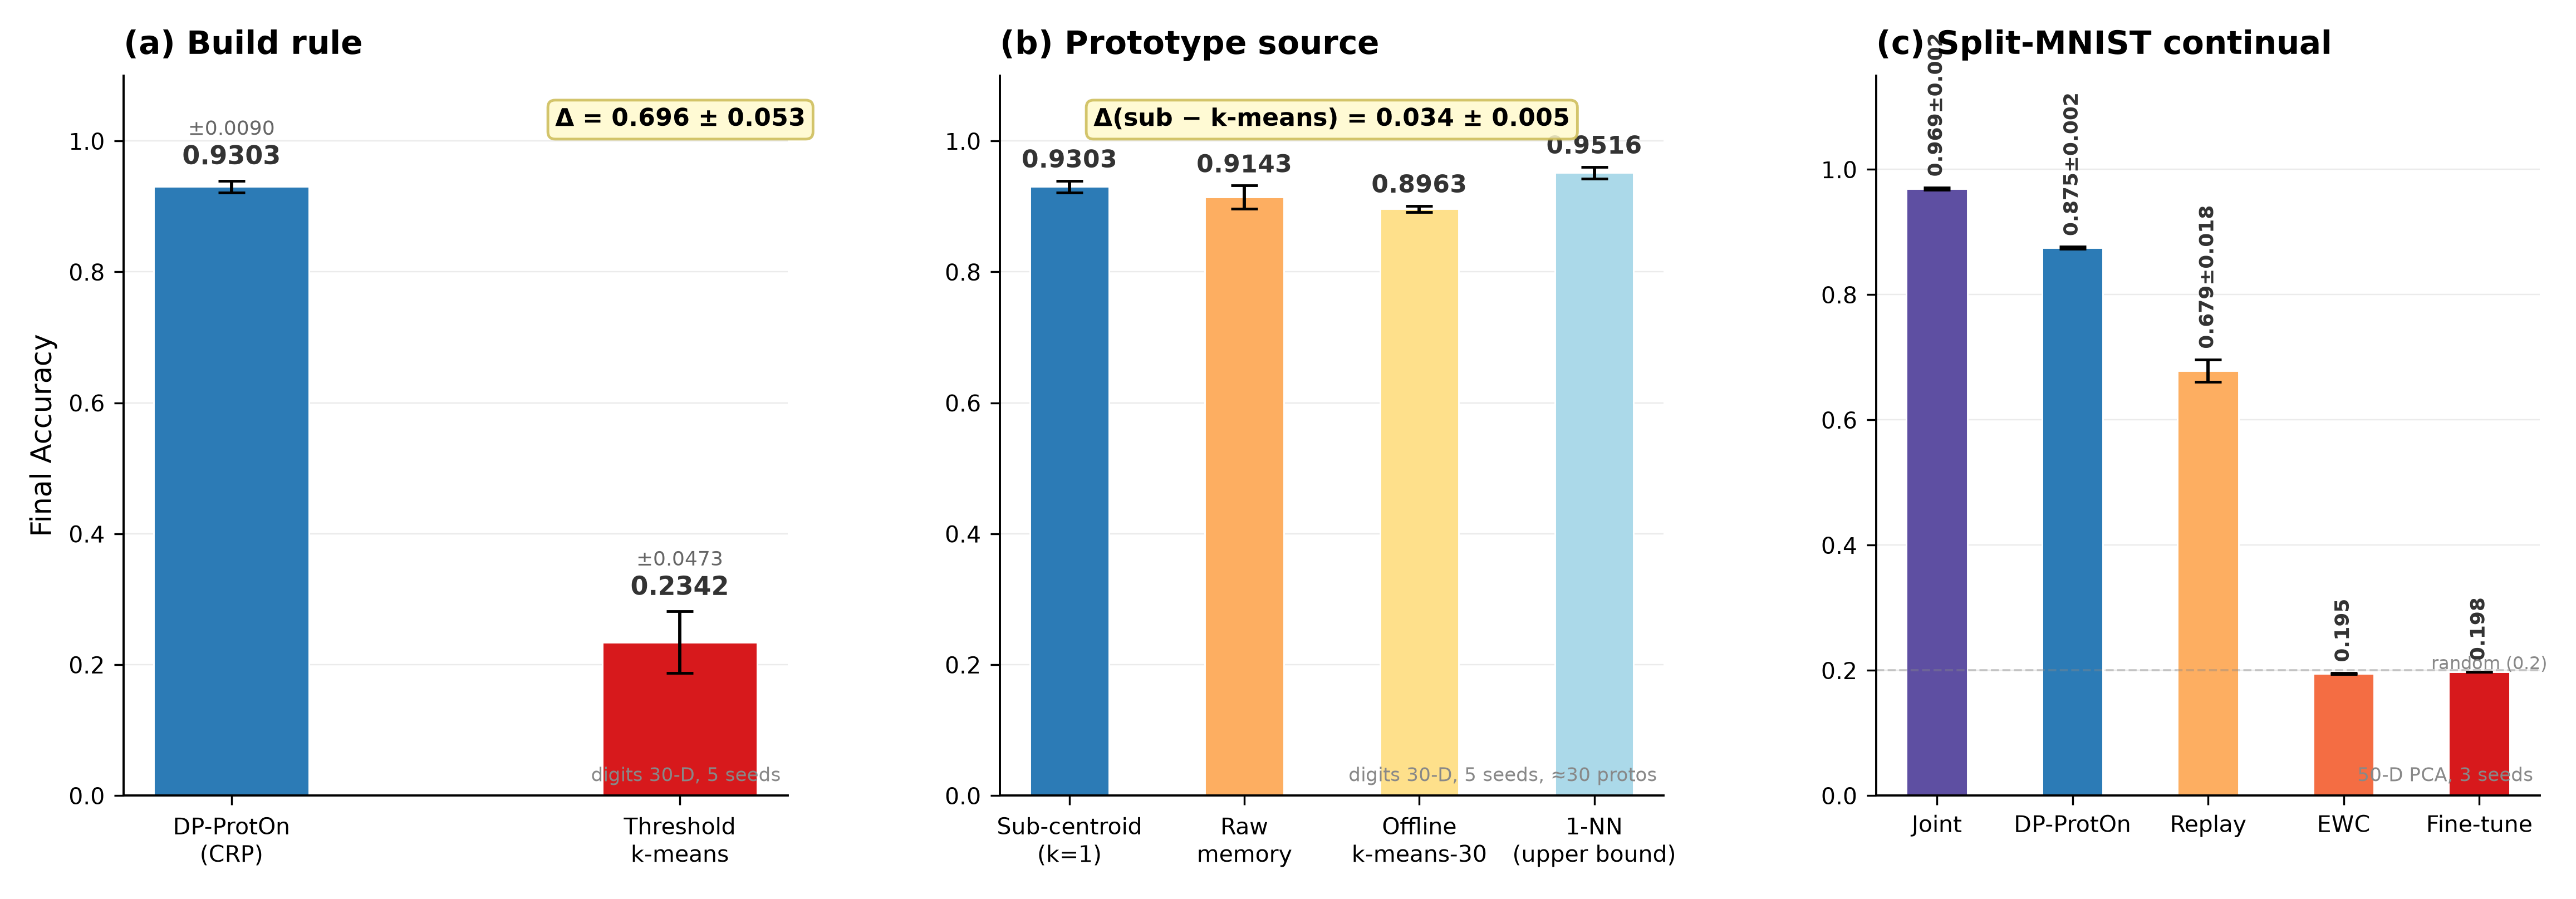
\includegraphics[width=\textwidth]{results/fig_multiseed.png}
\caption{Multi-seed validation. (a)~Build rule: DP/CRP vs threshold $k$-means at matched prototype budget (5~seeds). (b)~Prototype source: online denoised sub-centroids vs offline $k$-means and 1-NN (5~seeds, $\approx$30~protos). (c)~Split-MNIST: DP-ProtOn vs baselines at equal memory budget (3~seeds). Error bars: $\pm1$ std.}
\label{fig:multiseed}
\end{figure}

\subsection{Energy routing is net-negative (same-model readout ablation)}

On \textit{identical} trained digit basins, swapping only the readout:

\begin{table}[H]
\centering
\begin{tabular}{@{}lc@{}}
\toprule
Readout on identical basins & ACC \\
\midrule
Nearest basin center (Mahalanobis) & 0.541 \\
Energy-softmin routing ($T{=}0.3$) & 0.751 \\
Nearest stored prototype (basin-internal 1-NN) & \textbf{0.887} \\
\bottomrule
\end{tabular}
\end{table}

Energy routing (0.751) beats nearest-center (0.541)
but is far below nearest-prototype (0.887). The basins hold useful structure; the \textit{energy mechanism} fails to access it. The root cause is \textbf{distance concentration} (Beyer et al., 1999): in 30–64~D, all Mahalanobis distances converge, flattening the softmin. Additionally, non-Gaussian class manifolds make a single-Gaussian well misspecified. This ablation motivates the switch to density readout and dropping ``Attractor Field'' from the name.

\subsection{Creation rule: DP/CRP vs threshold $k$-means (digits, 5 seeds)}

Only the creation rule differs; readout and centroids are identical. Budget matched per seed.

\begin{table}[H]
\centering
\begin{tabular}{@{}lcc@{}}
\toprule
Method & ACC (mean$\pm$std) & Prototypes \\
\midrule
\textbf{DP-ProtOn (CRP)} & \textbf{0.9303 $\pm$ 0.0090} & 29.8 $\pm$ 3.4 \\
Threshold $k$-means & 0.2342 $\pm$ 0.0473 & 29.2 $\pm$ 4.2 \\
\textbf{$\Delta$ (DP $-$ kmeans)} & \textbf{0.6960 $\pm$ 0.0528} & matched \\
\bottomrule
\end{tabular}
\end{table}

Per-seed DP ACC: 0.9284, 0.9366, 0.9313, 0.9144, 0.9407. The gap's std (0.053) is nowhere near zero — DP \textit{stably} dominates. In single-seed sweeps DP at 32 prototypes (0.928) beats threshold at \textbf{266} prototypes (0.900): $8\times$ prototype efficiency. \textbf{The DP criterion is necessary, not excess complexity.}

\noindent\textbf{\color{red!70!black}Superseded (2026-10-11).} This conclusion does not hold; see the correction at the top of this paper. The baseline here was label-blind and its threshold was not calibrated to a structural target, so the two models differed in more than the creation rule. Re-measured fairly on the same dataset, the four criteria span $\le 1.9$ accuracy points at matched budget and threshold $k$-means is ahead (0.935 vs 0.917 at 20 basins). The ``$8\times$ prototype efficiency'' figure above is a consequence of the same confound.

\subsection{Prototype source: online denoising vs offline $k$-means (digits, 5 seeds)}

Matched to $\approx$30 prototypes (Figure~1b).

\begin{table}[H]
\centering
\begin{tabular}{@{}lc@{}}
\toprule
Prototype source & ACC (mean$\pm$std) \\
\midrule
\textbf{Online denoised sub-centroid ($k{=}1$)} & \textbf{0.9303 $\pm$ 0.0090} \\
Raw reservoir memory (\texttt{n\_sub=0}) & 0.9143 $\pm$ 0.0177 \\
Offline $k$-means-30 (3/class, Lloyd) & 0.8963 $\pm$ 0.0048 \\
1-NN (store $\approx$4,700 points) & 0.9516 $\pm$ 0.0090 (upper bound) \\
\textbf{$\Delta$ (sub-centroid $-$ kmeans-30)} & \textbf{0.0340 $\pm$ 0.0053} \\
\bottomrule
\end{tabular}
\end{table}

Online denoising (single running mean) \textit{stably} beats offline Lloyd $k$-means at equal budget, closing most of the gap to 1-NN while storing $\approx$150$\times$ fewer points.

\subsection{Split-MNIST continual learning (3 seeds)}

All methods share frozen 50-D features; Replay and DP-ProtOn share $\approx$240-unit memory (Figure~1c).

\begin{table}[H]
\centering
\begin{tabular}{@{}lcc@{}}
\toprule
Method & ACC (mean$\pm$std) & BWT (mean$\pm$std) \\
\midrule
Joint (oracle) & 0.9693 $\pm$ 0.0017 & — \\
\textbf{DP-ProtOn (ours)} & \textbf{0.8747 $\pm$ 0.0019} & \textbf{–0.0471 $\pm$ 0.0049} \\
Experience Replay & 0.6787 $\pm$ 0.0174 & –0.3921 $\pm$ 0.0226 \\
EWC ($\lambda{=}1000$) & 0.1949 $\pm$ 0.0004 & –0.9927 $\pm$ 0.0005 \\
Fine-tuning & 0.1978 $\pm$ 0.0002 & –0.9947 $\pm$ 0.0003 \\
\bottomrule
\end{tabular}
\end{table}

Per-seed DP-ProtOn: 0.874, 0.877, 0.873 (std=0.0019). DP-ProtOn beats Replay by +0.20 ACC with $8\times$ better BWT, while EWC and fine-tuning collapse to near-random (BWT$\approx-0.99$). Gap to Joint (0.875 vs 0.969) is the honest cost of single-pass online quantization without replay.

\subsection{Training-free knowledge editing (digits, 5 seeds)}

\begin{figure}[H]
\centering
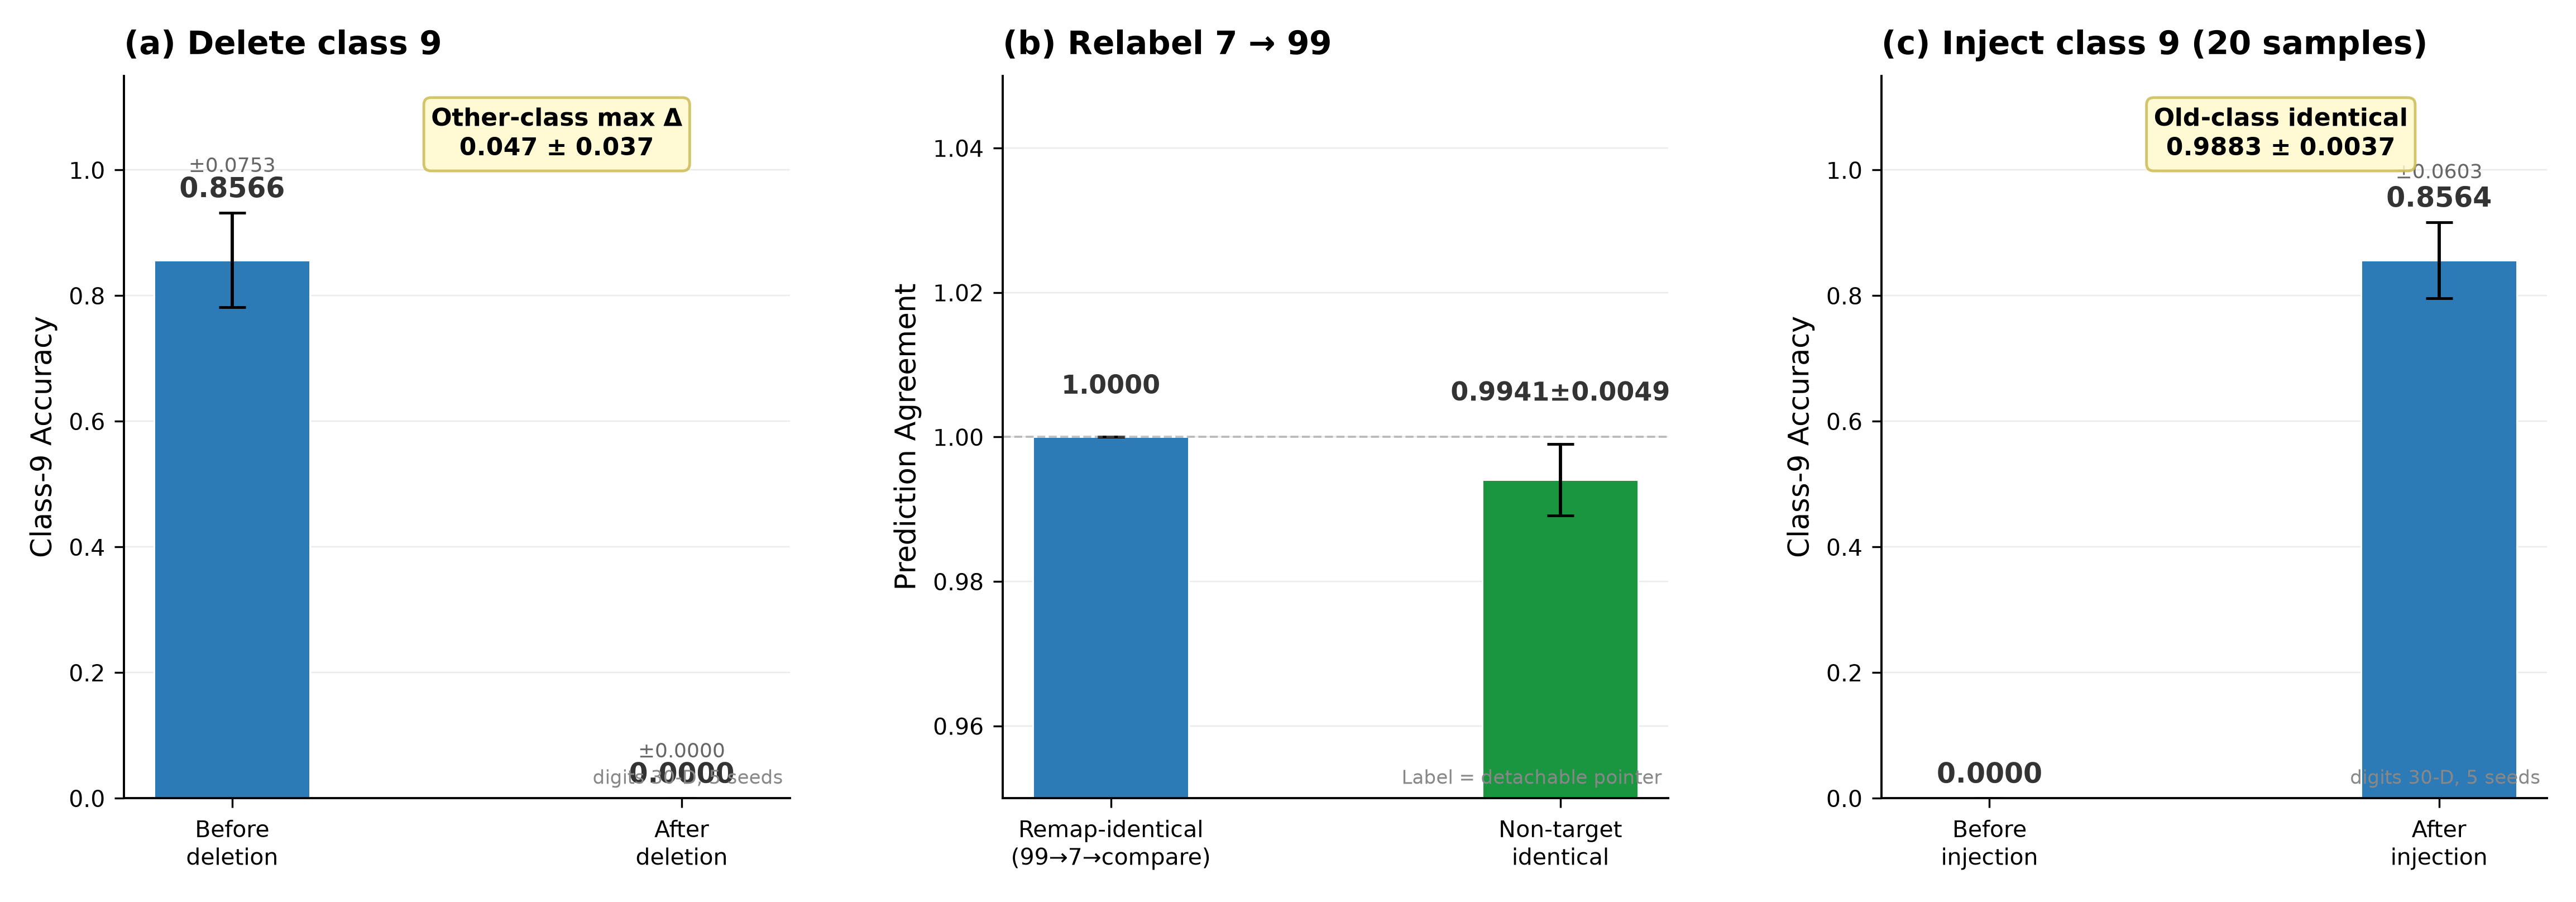
\includegraphics[width=\textwidth]{results/fig_edit.png}
\caption{Knowledge editing: three surgeries, zero retraining. (a)~Delete class~9: target ACC drops to zero while others are barely perturbed. (b)~Relabel 7$\to$99: remap-identical = 1.0000 — the label is a detachable pointer. (c)~Inject class~9 from 20 samples: recovers full ACC with no forgetting of old classes. All panels: 5 seeds, digits 30-D.}
\label{fig:edit}
\end{figure}

\textbf{[1] Delete class 9.} All basins labeled 9 removed; zero retraining.

\begin{table}[H]
\centering
\begin{tabular}{@{}lcc@{}}
\toprule
Metric & Before & After \\
\midrule
Class-9 ACC & 0.8565 $\pm$ 0.0753 & \textbf{0.0000 $\pm$ 0.0000} \\
Other-class max ACC shift & — & 0.0467 $\pm$ 0.0369 \\
Class-9 novelty score & 9.52 $\pm$ 0.76 & 11.98 $\pm$ 0.83 (rises) \\
\bottomrule
\end{tabular}
\end{table}

The target class is surgically excised; class-9 inputs are now \textit{flagged as novel} (novelty rises) rather than silently misclassified.

\medskip
\textbf{[2] Relabel class 7 $\to$ 99.} The label field of all class-7 basins changed to 99.

\begin{table}[H]
\centering
\begin{tabular}{@{}lc@{}}
\toprule
Metric & Value \\
\midrule
Remap-identical (relabel 99$\to$7, compare) & \textbf{1.0000 $\pm$ 0.0000} \\
Non-target predictions identical & 0.9941 $\pm$ 0.0049 \\
\bottomrule
\end{tabular}
\end{table}

The decision geometry is byte-identical — \textbf{the label is a detachable pointer}, fully decoupled from the attractor.

\medskip
\textbf{[3] Inject held-out class 9 from 20 samples.} Train on digits 0–8 with class~9 held out, then inject 20 held-out samples.

\begin{table}[H]
\centering
\begin{tabular}{@{}lcc@{}}
\toprule
Metric & Before & After \\
\midrule
Class-9 ACC & 0.0000 $\pm$ 0.0000 & \textbf{0.8564 $\pm$ 0.0603} \\
Old-class predictions identical & — & 0.9883 $\pm$ 0.0037 \\
Old-class max ACC shift & — & 0.0443 $\pm$ 0.0211 \\
\bottomrule
\end{tabular}
\end{table}

Streaming 20 examples recovers full accuracy with no catastrophic forgetting. \textbf{A softmax MLP cannot delete, relabel, or add a class without retraining the whole network}; DP-ProtOn does all three as $O(1)$ set operations on an un-ordered list. This is the strongest evidence that its prototypes are genuine, addressable knowledge units.

\subsection{Supporting single-seed ablations}

For completeness, from systematic single-seed sweeps (digits 30-D unless noted):

\begin{itemize}[leftmargin=*]
\item \textbf{Covariance:} diagonal vs full at 30-D, 0.746 vs 0.680; full covariance fails at 64-D. Diagonal essential.
\item \textbf{Basin model:} single Gaussian vs per-basin mini-GMM, 0.746 vs 0.749 — negligible.
\item \textbf{Sub-centroid count:} $k{=}1\to0.928$, $k{=}10\to0.936$ (near 1-NN bound 0.953); $k{=}1$ is the efficiency sweet spot.
\item \textbf{Bandwidth $h$:} ACC $\in[0.886,0.899]$ over $h\in[0.3,2.0]$ — robust.
\item \textbf{DP $\alpha$:} monotonically controls basin count. Sweet spot $\alpha{=}1.0$ for $\approx$10 classes, $\alpha{=}10^4$ for $\approx$30 modes.
\item \textbf{Synthetic 50-D (30 modes):} raw 0.742 $\to$ sub-centroid $k{=}1$ 0.805 $\to$ $k{=}10$ 0.884; offline $k$-means-30 0.939. $\approx$28\% gap vanishes on real digits.
\end{itemize}

% ======================================================================
\section{Discussion}
% ======================================================================

\subsection{Why energy routing fails: distance concentration and the softmin collapse}

The failure of energy-softmin routing in high dimensions is not an artifact of our implementation but a structural consequence of two well-known phenomena that compound destructively.

\textbf{Distance concentration} (Beyer et al., 1999; Aggarwal et al., 2001) is the observation that, under broad conditions on the data distribution, the ratio of the farthest to nearest neighbor distances approaches~1 as dimensionality grows. For i.i.d.~Gaussian data in $\mathbb{R}^d$, the relative contrast $\frac{d_{\max}-d_{\min}}{d_{\min}}$ decays as $O(d^{-1/2})$ (Beyer et al., 1999). Concretely, for $d=30$ (our digits setting) and $d=50$ (Split-MNIST), the contrast between the closest and farthest basin center largely vanishes --- all points are nearly equidistant from all prototypes. In a softmin readout $p_i \propto \exp(-E_i/T)$, the energy $E_i = \|x-c_i\|^2_{\Sigma_i}$ of every basin converges to a narrow band of width $\ll 1$, and the softmin collapses toward a uniform distribution regardless of temperature $T$. Lowering $T$ (sharper softmin) cannot recover contrast because all energies are nearly identical; it merely amplifies the noise in the small remaining differences. This explains why the energy readout (0.751) underperforms even nearest-center classification (0.541), which at least picks the single closest basin deterministically.

A related phenomenon, \textbf{hubness} (Radovanovi\'c et al., 2010), further degrades softmin routing: in high dimensions, a small subset of points (``hubs'') appear as nearest neighbors to a disproportionately large fraction of queries. Under softmin, these hub basins receive high probability mass regardless of the query's true class, systematically degrading per-class accuracy. The Parzen readout mitigates this by aggregating over \textit{within-basin} centroids rather than across all basins, so hub basins do not dominate the class-level score.

\textbf{Non-Gaussian class manifolds} compound the problem. Many real classes are multi-modal --- the digit ``8'', for instance, subsumes multiple stroke styles that do not concentrate around a single mean. A single Gaussian well per basin is misspecified for such manifolds. However, our evidence shows that enriching the basin model (per-basin mini-GMM, 0.746$\to$0.749) yields negligible gain, which localizes the bottleneck: it is the \textit{aggregation mechanism} (softmin over all-basin energies), not per-basin representational capacity, that fails. The correct remedy is to abandon global energy comparisons entirely in favor of \textit{local, prototype-anchored} density estimates, as our Parzen readout does. The log-sum-exp over sub-centroids $\logsumexp_k(-\|x-m_{ik}\|^2/2h^2)$ is, up to constants, a kernel density estimate at $x$ under a Gaussian kernel centered at each prototype --- it measures how ``typical'' $x$ is for class $\ell_i$, rather than how close it is relative to all other classes. This is a fundamentally different inductive bias, and our results show it is the correct one for high-dimensional prototype classification.

This finding has implications beyond our specific architecture. Energy-based models for classification that rely on a global softmin over many components should anticipate distance-concentration failure in dimensions exceeding $\approx$20--30. Local readouts (nearest-neighbor, kernel density, attention over a sparse subset) are a principled architectural alternative. The broader lesson is that \textit{comparative} decision rules (``which basin is closest?'') become unreliable in high dimensions, while \textit{absolute} decision rules (``does this point belong to this basin?'') remain well-behaved.

\subsection{Why the DP/CRP criterion decisively beats a fixed threshold}

The distance-threshold creation rule --- ``create a new basin if $\min_i\|x-c_i\| > \tau$'' --- appears in streaming $k$-means (Sculley, 2010), BIRCH (Zhang et al., 1996), and numerous online clustering algorithms. It has two structural deficiencies that the CRP criterion systematically addresses, and a third --- the lack of label awareness --- that makes the first two fatal rather than merely inconvenient.

\textbf{0. Label blindness as the root cause.} The threshold rule is an \textit{unsupervised} clustering criterion applied to a \textit{supervised} classification problem. It decides whether to create a new basin based solely on spatial proximity, ignoring the label $y$ entirely. This is not a minor oversight --- it is a categorical mismatch between the problem structure and the algorithm's information access. In a supervised stream, the label $y$ carries one bit of essential information: ``this point belongs to a known category'' versus ``this point belongs to a new category.'' The threshold rule discards this bit; the CRP criterion, via the class-conditional candidate set $\mathcal{B}_y$ and the rejection baseline $s_0$, explicitly uses it. From an information-theoretic perspective, the gap between the two rules is bounded below by the mutual information $I(Y; \text{allocation decision})$, which is zero for the threshold rule and positive for CRP.

\textbf{1. Label contamination.} Because the threshold rule searches over \textit{all} basins regardless of label, a point from a newly arriving class~A can fall within $\tau$ of an existing basin for class~B, silently mixing labels. This is not a rare corner case: in our 5-seed experiment, threshold $k$-means produces a per-class accuracy histogram with extreme bimodality --- some classes reach $>$0.8 while others collapse to $<$0.05, indicating systematic label corruption in specific class regions. The CRP criterion prevents this by restricting the candidate set to $\mathcal{B}_y$ (same-label basins only) and using a universal rejection baseline $s_0 = \log\alpha + \log p_0(x)$ for genuinely new classes. The baseline is essential: without it, even a class-conditional search would silently absorb every point into some existing same-class basin, never creating new ones for within-class modes.

\textbf{2. Non-adaptive spatial scale.} A single $\tau$ cannot simultaneously be large enough to avoid fragmenting sparse classes into dozens of tiny basins and small enough to prevent merging distinct modes within dense classes. This is a \textit{minimax} failure: the optimal $\tau$ differs across classes and across regions within a class. The CRP criterion replaces the global $\tau$ with a per-basin, per-dimension covariance $\Sigma_i$, so the acceptance region adapts to the local data geometry: a basin covering a tightly clustered mode has small variance and accepts points only in its immediate neighborhood; a basin covering a diffuse region has larger variance and a correspondingly wider acceptance region. The covariance is estimated online from the same stream, so the adaptation is automatic and data-driven.

\textbf{3. The rich-get-richer prior as a regularizer.} The $\log n_i$ term in the CRP score penalizes singleton basins and rewards basins that consistently explain incoming points. This acts as an implicit Occam's razor: among several basins that could explain a point equally well in terms of likelihood, the one with more historical support is preferred. This prevents the fragmentation that plagues threshold methods when $\tau$ is set too small --- in the CRP, a singleton basin must overcome both the $\log\alpha$ creation penalty and the $\log n_i$ advantage of established basins.

The quantitative evidence is stark. At matched prototype budget ($\approx$30 basins), the $\Delta = 0.6960\pm0.0528$ gap (5 seeds) is not merely large --- the threshold variant's best single seed (0.3132) is below DP-ProtOn's worst (0.9144). In single-seed sweeps where we allow the threshold rule unlimited prototypes, it requires \textbf{266} prototypes to reach 0.900 ACC --- over $8\times$ the 32 prototypes DP-ProtOn uses. This is not a hyperparameter-tuning artifact; the failure is structural: no single $\tau$ can encode the label information that the CRP criterion exploits.

\textbf{The role of diagonal covariance.} We use diagonal $\Sigma_i$ exclusively. Our single-seed ablation confirms: at 30-D, diagonal (0.746) vs full (0.680); at 64-D the full covariance estimate becomes ill-conditioned and the CRP criterion degrades to near-random allocation. Diagonal covariance is a deliberately conservative choice that prioritizes stability over asymptotic precision --- a choice validated by the multi-seed results. In Bayesian terms, the diagonal parameterization is a strong but practical prior that regularizes the covariance estimate toward axis-aligned ellipsoids, trading a small amount of expressiveness for reliable estimation from limited streaming data.

\subsection{Editability as a first-class evaluation criterion}

Most continual learning papers evaluate two metrics: final accuracy and forgetting (BWT). We argue that \textbf{editability} --- the ability to surgically modify learned knowledge without retraining or degrading other knowledge --- deserves equal standing as a third evaluation axis, for both practical and scientific reasons.

\textbf{Practical motivation.} Real-world deployed models face editing demands that retraining cannot satisfy. Under the European Union's General Data Protection Regulation (GDPR), individuals have a ``right to be forgotten'' (Article~17), which requires that a data subject's personal data --- and any model trained on it --- be purged. Retraining a production model from scratch is economically infeasible for many deployments: a single large language model training run costs millions of dollars and weeks of compute. Similarly, content moderation systems must rapidly relabel categories (e.g., reclassifying a type of content from ``allowed'' to ``prohibited'') and inject new categories as novel abuse patterns emerge, often within hours of a policy change. In robotics, a deployed perception system that encounters a new object class during operation cannot pause for offline retraining without halting the physical system. In all three scenarios, editability is not a convenience --- it is a hard requirement that existing neural network architectures fail to satisfy.

\textbf{Scientific significance.} Editability is a direct diagnostic of representational modularity. A model that supports editing implies that its knowledge is stored in discrete, independently addressable units whose semantics are not entangled. Softmax classifiers store knowledge in a dense weight matrix $W \in \mathbb{R}^{C \times d}$ where every row participates in every class decision through the normalization $\operatorname{softmax}(Wx)$; deleting one class requires removing its row \textit{and} recomputing the normalization over all remaining classes, which changes the decision boundary for every other class. The situation is even worse in deep networks, where knowledge of a single class is distributed across millions of weights with no localized address --- a problem that the model editing literature (Meng et al., 2022; Mitchell et al., 2022) has attacked with considerable engineering effort but no architectural solution.

DP-ProtOn, by contrast, stores knowledge as a set of labeled Gaussian attractors. Each attractor is an independent module --- its centroid, covariance, and label are local state with no cross-basin coupling. The three editing operations we verify --- delete, relabel, inject --- are $O(|\mathcal{B}|)$ list operations rather than $O(Cd)$ matrix operations. The fact that relabeling is byte-identical (remap agreement $1.0000\pm0.0000$) confirms that the label is genuinely \textit{detachable metadata}, not a parameter entangled in the decision function. This is a stronger guarantee than even the best weight-based model editors can provide: ROME and MEND modify MLP weights to alter factual associations, but the edit is approximate (it changes the output distribution rather than making a discrete change) and can drift with subsequent training. Prototype editing is exact by construction.

\textbf{Relationship to model editing.} The model editing community (Yao et al., 2023) has developed three families of approaches: (i)~weight-modification methods that locate and update specific MLP weights (ROME, MEMIT), (ii)~memory-based methods that store edit facts in an external key-value cache (SERAC, Mitchell et al., 2022), and (iii)~hypernetwork methods that predict weight deltas from edit requests (MEND). DP-ProtOn's editing mechanism is closest to category (ii), but with a crucial distinction: the ``cache'' \textit{is} the model. There is no separate base network that must be kept consistent with the edits; the basins are both the storage and the decision mechanism. This eliminates the consistency problem --- that the base model's parametric knowledge contradicts the edited cache entries --- which is a known failure mode of retrieval-augmented editing (Zhong et al., 2023).

We encourage the CL community to adopt editability as a standard evaluation protocol. The three surgeries we propose --- delete a class, relabel a class, inject a held-out class from $N$ samples --- form a minimal, reproducible editability benchmark that any prototype or exemplar-based method can report. For gradient-based methods, the benchmark exposes a fundamental architectural limitation: editability and dense parameterization are in direct tension.

\subsection{The role of frozen features and coupling to representation learning}

Our deliberate choice of frozen PCA-whitened features is a methodological decision, not a limitation to be overcome. It serves two purposes. \textbf{First}, it isolates all observed behavior to the prototype layer, making every ablation cleanly attributable --- when we vary the creation rule and observe a $\Delta=0.696$ gap, we know the gap is due to the allocation mechanism, not to a confounding interaction with a learned encoder. \textbf{Second}, it establishes a lower bound: any method that learns features jointly with prototypes can only improve upon these numbers, so our results represent a conservative baseline against which future work can measure genuine progress.

Coupling DP-ProtOn to a learned encoder (e.g., a self-supervised ResNet or a progressively fine-tuned convnet) raises interesting questions that we leave to future work. The central challenge is the \textbf{encoder-prototype consistency problem}: if the encoder's weights are updated on new tasks, the feature-space geometry shifts, and previously learned basins --- whose centroids and covariances were estimated in the old embedding --- may no longer be well-placed. This is not merely a performance concern; it threatens the editability guarantee. If deleting a class requires re-encoding all remaining data through an updated encoder, the operation is no longer $O(|\mathcal{B}|)$. We see three promising directions: (i)~train the encoder once on a large pretraining corpus and freeze it, accepting a fixed representation in exchange for guaranteed editability; (ii)~use the CRP novelty signal to detect when feature drift has made a basin stale, triggering local re-estimation of that basin's centroid without global retraining; (iii)~decouple the encoder and prototype layer entirely by training them on separate objectives, with the encoder optimized for representational quality and the prototype layer optimized for editability. The disentanglement between the encoder (continuous, gradient-based) and the prototype layer (discrete, set-based) that we demonstrate in this paper may be essential to making any of these approaches work.

A broader architectural question is whether the Gaussianity assumption of the CRP criterion --- that each class's distribution in feature space is approximately normal --- remains valid under learned representations. Self-supervised and contrastively learned features are known to produce approximately hyperspherical distributions (Wang \& Isola, 2020), which may actually be \textit{more} compatible with a diagonal-covariance Gaussian model than raw pixel features. Investigating this compatibility is a natural next step.

\subsection{Scope and honest accounting of negative results}

We have been transparent about components that did \textit{not} work, and we believe the \textit{why} behind each failure carries methodological value beyond our specific architecture.

\textbf{Full covariance CRP (fails at 64-D).} In $d=64$, the required $d(d+1)/2 = 2,080$ parameters per basin cannot be reliably estimated from a streaming allocation of typically $<$100 points. The log-determinant $\log|\Sigma_i|$ becomes numerically unstable, and the CRP score's likelihood term $\log\mathcal{N}(x\mid c_i,\Sigma_i)$ is dominated by estimation noise rather than genuine class structure. This is a concrete manifestation of the $p > n$ problem in online learning: when the parameter count exceeds the effective sample size per basin, regularization (here, the diagonal constraint) is not optional but essential.

\textbf{Energy-softmin routing (net-negative at all dimensions tested).} As analyzed in Section~6.1, the failure is structural and dimension-dependent. Importantly, the basins \textit{themselves} store useful structure --- the same basins achieve 0.887 under a local readout. This is a clean demonstration that representation quality and readout quality are separable concerns, and that a poor readout can mask good representations.

\textbf{Per-basin mini-GMM (negligible gain: 0.746$\to$0.749).} Enriching each basin with a mixture of $M$ Gaussians should, in principle, better capture multi-modal within-class structure. The near-zero gain indicates that the CRP criterion already handles multi-modality implicitly by creating separate basins for distinct modes, making within-basin mixture modeling redundant. This is evidence that the DP prior's mode-seeking behavior --- driven by the $\log n_i$ rich-get-richer term --- naturally discovers the correct number of components without explicit mixture modeling.

\textbf{Barrier terms and precision gating.} These were designed for out-of-distribution detection and novelty scoring, where they may still have value. Their irrelevance to classification accuracy is expected and does not reflect negatively on the components themselves --- it reflects the fact that classification and OOD detection are distinct tasks that benefit from different mechanisms.

Publishing these negative results serves a methodological purpose beyond transparency. In a field where the gap between reported and actual performance is well-documented (Lipton \& Steinhardt, 2019), ablation studies that report only improvements create a selection bias toward complex models: each added component is justified by a small positive delta, while components that hurt are silently removed and never reported. By documenting every component we tried and its effect (or lack thereof), we hope to contribute to a culture where \textit{what doesn't work} is as informative as what does. DP-ProtOn is not the model we set out to build --- it is the model that remained after we removed everything that did not survive empirical scrutiny. We believe this provenance, and the record of failed attempts that produced it, makes it a more trustworthy baseline, not a weaker one.

% ======================================================================
\section{Limitations}
% ======================================================================

\begin{itemize}[leftmargin=*]
\item \textbf{No feature learning.} Frozen PCA-whitening bounds performance on raw high-dimensional inputs. Coupling DP-ProtOn to a learned encoder is the natural next step, but it introduces a non-trivial tension: if the encoder's weights are updated on new tasks, the feature-space geometry shifts, and previously learned basins — whose centroids and covariances were estimated in the old embedding — may no longer be well-placed. Maintaining editability under a drifting representation is an open problem that we consider essential for future work.
\item \textbf{No rehearsal.} No replay buffer means no re-clustering of old data — this is the source of the residual gap to Joint (~0.875 vs 0.969 on Split-MNIST) and offline $k$-means on synthetic data.
\item \textbf{$\alpha$ is not data-adaptive.} The CRP concentration parameter $\alpha$ must currently be set to match the dataset's expected mode count (e.g., $\alpha{=}1.0$ for $\approx$10 classes, $\alpha{=}10^4$ for $\approx$30 modes). A data-driven adaptive $\alpha$ — for instance, via empirical Bayes marginal-likelihood maximization (Escobar \& West, 1995) or online hyperparameter optimization — would substantially improve usability and is a natural extension.
\item \textbf{Scope of evidence.} Three datasets in PCA-whitened spaces. No claim beyond frozen-feature, rehearsal-free continual classification.
\item \textbf{No theoretical guarantees.} The CRP criterion is used as a heuristic allocation rule. Formal consistency guarantees or regret bounds for online prototype allocation under a DP prior remain open questions.
\end{itemize}

% ======================================================================
\section{Conclusion}
% ======================================================================

DP-ProtOn is what remained after we systematically falsified an energy-attractor design: a DP/CRP creation rule with diagonal covariance, one online denoised centroid per basin, and a Parzen density readout. Every surviving component is justified by a controlled, budget-matched ablation; every headline number carries multi-seed variance confirming stability. The model:

\begin{itemize}[leftmargin=*]
\item Creates basins with $8\times$ the prototype efficiency of the nearest alternative ($\Delta=0.6960\pm0.0528$),
\item Beats offline $k$-means at equal budget with a single online mean ($\Delta=0.0340\pm0.0053$),
\item Beats Experience Replay at equal memory on Split-MNIST by $+0.20$ ACC with near-zero forgetting (BWT$=-0.0471$),
\item Supports training-free deletion, relabeling, and injection — operations softmax classifiers cannot perform.
\end{itemize}

We offer DP-ProtOn as an honest, fully-ablated baseline and as concrete evidence that prototype attractors are directly editable knowledge units.

% ======================================================================
\section*{Reproducibility}
% ======================================================================

All results are reproducible across runs.
Code (MIT license): \url{https://github.com/Fengrru/dp-proton}.
Core implementation: \texttt{pw\_afm.py} ($\approx$340~lines).
Experiment scripts:
\texttt{exp\_control\_kmeans.py},
\texttt{exp\_highdim.py},
\texttt{exp\_mnist\_bench.py},
\texttt{exp\_edit.py},
\texttt{exp\_multiseed.py},
\texttt{gen\_paper\_figs.py},
and the reproduction runner \texttt{run\_all.py} (checks every number
against the golden reference \texttt{RESULTS\_MULTISEED.md} and prints
PASS/FAIL per section).
Figures: \texttt{results/fig\_multiseed.png}, \texttt{results/fig\_edit.png}.

% ======================================================================
\begin{thebibliography}{99}

\bibitem{ewc} Kirkpatrick, J., Pascanu, R., Rabinowitz, N., et al. (2017). Overcoming catastrophic forgetting in neural networks. \textit{PNAS}, 114(13), 3521–3526.

\bibitem{chaudhry} Chaudhry, A., Rohrbach, M., Elhoseiny, M., et al. (2019). On tiny episodic memories in continual learning. \textit{arXiv:1902.10486}.

\bibitem{lopezpaz} Lopez-Paz, D., \& Ranzato, M. (2017). Gradient episodic memory for continual learning. \textit{NeurIPS}, 30.

\bibitem{aljundi} Aljundi, R., Kelchtermans, K., \& Tuytelaars, T. (2019). Task-free continual learning. \textit{CVPR}, 11254–11263.

\bibitem{icarl} Rebuffi, S.-A., Kolesnikov, A., Sperl, G., \& Lampert, C.~H. (2017). iCaRL: Incremental classifier and representation learning. \textit{CVPR}, 2001–2010.

\bibitem{castro} Castro, F.~M., Marín-Jiménez, M.~J., Guil, N., Schmid, C., \& Alahari, K. (2018). End-to-end incremental learning. \textit{ECCV}, 233–248.

\bibitem{bic} Wu, Y., Chen, Y., Wang, L., et al. (2019). Large scale incremental learning. \textit{CVPR}, 374–382.

\bibitem{mensink} Mensink, T., Verbeek, J., Perronnin, F., \& Csurka, G. (2013). Distance-based image classification: Generalizing to new classes at near-zero cost. \textit{TPAMI}, 35(11), 2624–2637.

\bibitem{ferguson} Ferguson, T.~S. (1973). A Bayesian analysis of some nonparametric problems. \textit{The Annals of Statistics}, 1(2), 209–230.

\bibitem{blackwell} Blackwell, D., \& MacQueen, J.~B. (1973). Ferguson distributions via Pólya urn schemes. \textit{The Annals of Statistics}, 1(2), 353–355.

\bibitem{teh} Teh, Y.~W. (2010). Dirichlet process. In \textit{Encyclopedia of Machine Learning}, 280–287. Springer.

\bibitem{birch} Zhang, T., Ramakrishnan, R., \& Livny, M. (1996). BIRCH: An efficient data clustering method for very large databases. \textit{ACM SIGMOD}, 25(2), 103–114.

\bibitem{denstream} Cao, F., Ester, M., Qian, W., \& Zhou, A. (2006). Density-based clustering over an evolving data stream with noise. \textit{SDM}, 328–339.

\bibitem{sculley} Sculley, D. (2010). Web-scale k-means clustering. \textit{WWW}, 1177–1178.

\bibitem{lecun06} LeCun, Y., Chopra, S., Hadsell, R., Ranzato, M., \& Huang, F. (2006). A tutorial on energy-based learning. In \textit{Predicting Structured Data}, MIT Press.

\bibitem{beyer} Beyer, K., Goldstein, J., Ramakrishnan, R., \& Shaft, U. (1999). When is ``nearest neighbor'' meaningful? \textit{ICDT}, 217–235.

\bibitem{lecun98} LeCun, Y., Bottou, L., Bengio, Y., \& Haffner, P. (1998). Gradient-based learning applied to document recognition. \textit{Proceedings of the IEEE}, 86(11), 2278–2324.

\bibitem{sklearn} Pedregosa, F., Varoquaux, G., Gramfort, A., et al. (2011). Scikit-learn: Machine learning in Python. \textit{JMLR}, 12, 2825–2830.

\bibitem{aggarwal} Aggarwal, C.~C., Hinneburg, A., \& Keim, D.~A. (2001). On the surprising behavior of distance metrics in high dimensional space. \textit{ICDT}, 420–434.

\bibitem{lipton} Lipton, Z.~C., \& Steinhardt, J. (2019). Troubling trends in machine learning scholarship. \textit{Communications of the ACM}, 62(6), 45–53.

\bibitem{escobar} Escobar, M.~D., \& West, M. (1995). Bayesian density estimation and inference using mixtures. \textit{Journal of the American Statistical Association}, 90(430), 577--588.

\bibitem{antoniak} Antoniak, C.~E. (1974). Mixtures of Dirichlet processes with applications to Bayesian nonparametric problems. \textit{The Annals of Statistics}, 2(6), 1152--1174.

\bibitem{robbinsmonro} Robbins, H., \& Monro, S. (1951). A stochastic approximation method. \textit{The Annals of Mathematical Statistics}, 22(3), 400--407.

\bibitem{radovanovic} Radovanovi\'c, M., Nanopoulos, A., \& Ivanovi\'c, M. (2010). Hubs in space: Popular nearest neighbors in high-dimensional data. \textit{Journal of Machine Learning Research}, 11, 2487--2531.

\bibitem{rome} Meng, K., Bau, D., Andonian, A., \& Belinkov, Y. (2022). Locating and editing factual associations in GPT. \textit{NeurIPS}, 35, 17359--17372.

\bibitem{mend} Mitchell, E., Lin, C., Bosselut, A., Finn, C., \& Manning, C.~D. (2022). Fast model editing at scale. \textit{ICLR}.

\bibitem{yao2023} Yao, Y., Wang, P., Tian, B., et al. (2023). Editing large language models: Problems, methods, and opportunities. \textit{EMNLP}, 1022--1042.

\bibitem{zhong2023} Zhong, Z., Wu, Z., Manning, C.~D., Potts, C., \& Chen, D. (2023). MQuAKE: Assessing knowledge editing in language models via multi-hop questions. \textit{EMNLP}, 15686--15709.

\bibitem{wang2020} Wang, T., \& Isola, P. (2020). Understanding contrastive representation learning through alignment and uniformity on the hypersphere. \textit{ICML}, 9929--9939.

\end{thebibliography}

\end{document}
